\documentclass[12pt,a4paper]{article}

\usepackage[a4paper,text={16.5cm,25.2cm},centering]{geometry}
\usepackage{lmodern}
\usepackage{amssymb,amsmath}
\usepackage{bm}
\usepackage{graphicx}
\usepackage{microtype}
\usepackage{hyperref}
\setlength{\parindent}{0pt}
\setlength{\parskip}{1.2ex}

\hypersetup
       {   pdfauthor = { Sheehan Olver },
           pdftitle={ foo },
           colorlinks=TRUE,
           linkcolor=black,
           citecolor=blue,
           urlcolor=blue
       }




\usepackage{upquote}
\usepackage{listings}
\usepackage{xcolor}
\lstset{
    basicstyle=\ttfamily\footnotesize,
    upquote=true,
    breaklines=true,
    breakindent=0pt,
    keepspaces=true,
    showspaces=false,
    columns=fullflexible,
    showtabs=false,
    showstringspaces=false,
    escapeinside={(*@}{@*)},
    extendedchars=true,
}
\newcommand{\HLJLt}[1]{#1}
\newcommand{\HLJLw}[1]{#1}
\newcommand{\HLJLe}[1]{#1}
\newcommand{\HLJLeB}[1]{#1}
\newcommand{\HLJLo}[1]{#1}
\newcommand{\HLJLk}[1]{\textcolor[RGB]{148,91,176}{\textbf{#1}}}
\newcommand{\HLJLkc}[1]{\textcolor[RGB]{59,151,46}{\textit{#1}}}
\newcommand{\HLJLkd}[1]{\textcolor[RGB]{214,102,97}{\textit{#1}}}
\newcommand{\HLJLkn}[1]{\textcolor[RGB]{148,91,176}{\textbf{#1}}}
\newcommand{\HLJLkp}[1]{\textcolor[RGB]{148,91,176}{\textbf{#1}}}
\newcommand{\HLJLkr}[1]{\textcolor[RGB]{148,91,176}{\textbf{#1}}}
\newcommand{\HLJLkt}[1]{\textcolor[RGB]{148,91,176}{\textbf{#1}}}
\newcommand{\HLJLn}[1]{#1}
\newcommand{\HLJLna}[1]{#1}
\newcommand{\HLJLnb}[1]{#1}
\newcommand{\HLJLnbp}[1]{#1}
\newcommand{\HLJLnc}[1]{#1}
\newcommand{\HLJLncB}[1]{#1}
\newcommand{\HLJLnd}[1]{\textcolor[RGB]{214,102,97}{#1}}
\newcommand{\HLJLne}[1]{#1}
\newcommand{\HLJLneB}[1]{#1}
\newcommand{\HLJLnf}[1]{\textcolor[RGB]{66,102,213}{#1}}
\newcommand{\HLJLnfm}[1]{\textcolor[RGB]{66,102,213}{#1}}
\newcommand{\HLJLnp}[1]{#1}
\newcommand{\HLJLnl}[1]{#1}
\newcommand{\HLJLnn}[1]{#1}
\newcommand{\HLJLno}[1]{#1}
\newcommand{\HLJLnt}[1]{#1}
\newcommand{\HLJLnv}[1]{#1}
\newcommand{\HLJLnvc}[1]{#1}
\newcommand{\HLJLnvg}[1]{#1}
\newcommand{\HLJLnvi}[1]{#1}
\newcommand{\HLJLnvm}[1]{#1}
\newcommand{\HLJLl}[1]{#1}
\newcommand{\HLJLld}[1]{\textcolor[RGB]{148,91,176}{\textit{#1}}}
\newcommand{\HLJLs}[1]{\textcolor[RGB]{201,61,57}{#1}}
\newcommand{\HLJLsa}[1]{\textcolor[RGB]{201,61,57}{#1}}
\newcommand{\HLJLsb}[1]{\textcolor[RGB]{201,61,57}{#1}}
\newcommand{\HLJLsc}[1]{\textcolor[RGB]{201,61,57}{#1}}
\newcommand{\HLJLsd}[1]{\textcolor[RGB]{201,61,57}{#1}}
\newcommand{\HLJLsdB}[1]{\textcolor[RGB]{201,61,57}{#1}}
\newcommand{\HLJLsdC}[1]{\textcolor[RGB]{201,61,57}{#1}}
\newcommand{\HLJLse}[1]{\textcolor[RGB]{59,151,46}{#1}}
\newcommand{\HLJLsh}[1]{\textcolor[RGB]{201,61,57}{#1}}
\newcommand{\HLJLsi}[1]{#1}
\newcommand{\HLJLso}[1]{\textcolor[RGB]{201,61,57}{#1}}
\newcommand{\HLJLsr}[1]{\textcolor[RGB]{201,61,57}{#1}}
\newcommand{\HLJLss}[1]{\textcolor[RGB]{201,61,57}{#1}}
\newcommand{\HLJLssB}[1]{\textcolor[RGB]{201,61,57}{#1}}
\newcommand{\HLJLnB}[1]{\textcolor[RGB]{59,151,46}{#1}}
\newcommand{\HLJLnbB}[1]{\textcolor[RGB]{59,151,46}{#1}}
\newcommand{\HLJLnfB}[1]{\textcolor[RGB]{59,151,46}{#1}}
\newcommand{\HLJLnh}[1]{\textcolor[RGB]{59,151,46}{#1}}
\newcommand{\HLJLni}[1]{\textcolor[RGB]{59,151,46}{#1}}
\newcommand{\HLJLnil}[1]{\textcolor[RGB]{59,151,46}{#1}}
\newcommand{\HLJLnoB}[1]{\textcolor[RGB]{59,151,46}{#1}}
\newcommand{\HLJLoB}[1]{\textcolor[RGB]{102,102,102}{\textbf{#1}}}
\newcommand{\HLJLow}[1]{\textcolor[RGB]{102,102,102}{\textbf{#1}}}
\newcommand{\HLJLp}[1]{#1}
\newcommand{\HLJLc}[1]{\textcolor[RGB]{153,153,119}{\textit{#1}}}
\newcommand{\HLJLch}[1]{\textcolor[RGB]{153,153,119}{\textit{#1}}}
\newcommand{\HLJLcm}[1]{\textcolor[RGB]{153,153,119}{\textit{#1}}}
\newcommand{\HLJLcp}[1]{\textcolor[RGB]{153,153,119}{\textit{#1}}}
\newcommand{\HLJLcpB}[1]{\textcolor[RGB]{153,153,119}{\textit{#1}}}
\newcommand{\HLJLcs}[1]{\textcolor[RGB]{153,153,119}{\textit{#1}}}
\newcommand{\HLJLcsB}[1]{\textcolor[RGB]{153,153,119}{\textit{#1}}}
\newcommand{\HLJLg}[1]{#1}
\newcommand{\HLJLgd}[1]{#1}
\newcommand{\HLJLge}[1]{#1}
\newcommand{\HLJLgeB}[1]{#1}
\newcommand{\HLJLgh}[1]{#1}
\newcommand{\HLJLgi}[1]{#1}
\newcommand{\HLJLgo}[1]{#1}
\newcommand{\HLJLgp}[1]{#1}
\newcommand{\HLJLgs}[1]{#1}
\newcommand{\HLJLgsB}[1]{#1}
\newcommand{\HLJLgt}[1]{#1}



\def\qqand{\qquad\hbox{and}\qquad}
\def\qqfor{\qquad\hbox{for}\qquad}
\def\qqas{\qquad\hbox{as}\qquad}
\def\half{ {1 \over 2} }
\def\D{ {\rm d} }
\def\I{ {\rm i} }
\def\E{ {\rm e} }
\def\C{ {\mathbb C} }
\def\R{ {\mathbb R} }
\def\CC{ {\cal C} }
\def\HH{ {\cal H} }
\def\LL{ {\cal L} }
\def\vc#1{ {\mathbf #1} }
\def\bbC{ {\mathbb C} }

\def\qqqquad{\qquad\qquad}
\def\qqwhere{\qquad\hbox{where}\qquad}
\def\Res_#1{\underset{#1}{\rm Res}\,}
\def\sech{ {\rm sech}\, }
\def\acos{ {\rm acos}\, }
\def\atan{ {\rm atan}\, }
\def\upepsilon{\varepsilon}


\def\Xint#1{ \mathchoice
   {\XXint\displaystyle\textstyle{#1} }%
   {\XXint\textstyle\scriptstyle{#1} }%
   {\XXint\scriptstyle\scriptscriptstyle{#1} }%
   {\XXint\scriptscriptstyle\scriptscriptstyle{#1} }%
   \!\int}
\def\XXint#1#2#3{ {\setbox0=\hbox{$#1{#2#3}{\int}$}
     \vcenter{\hbox{$#2#3$}}\kern-.5\wd0} }
\def\ddashint{\Xint=}
\def\dashint{\Xint-}
% \def\dashint
\def\infdashint{\dashint_{-\infty}^\infty}




\def\addtab#1={#1\;&=}
\def\ccr{\\\addtab}
\def\ip<#1>{\left\langle{#1}\right\rangle}
\def\dx{\D x}
\def\dt{\D t}
\def\dz{\D z}

\def\norm#1{\left\| #1 \right\|}

\def\pr(#1){\left({#1}\right)}
\def\br[#1]{\left[{#1}\right]}

\def\abs#1{\left|{#1}\right|}
\def\fpr(#1){\!\pr({#1})}

\def\sopmatrix#1{ \begin{pmatrix}#1\end{pmatrix} }

\def\endash{–}
\def\mdblksquare{\blacksquare}
\def\lgblksquare{\blacksquare}
\def\scre{\E}
\def\mapengine#1,#2.{\mapfunction{#1}\ifx\void#2\else\mapengine #2.\fi }

\def\map[#1]{\mapengine #1,\void.}

\def\mapenginesep_#1#2,#3.{\mapfunction{#2}\ifx\void#3\else#1\mapengine #3.\fi }

\def\mapsep_#1[#2]{\mapenginesep_{#1}#2,\void.}


\def\vcbr[#1]{\pr(#1)}


\def\bvect[#1,#2]{
{
\def\dots{\cdots}
\def\mapfunction##1{\ | \  ##1}
	\sopmatrix{
		 \,#1\map[#2]\,
	}
}
}



\def\vect[#1]{
{\def\dots{\ldots}
	\vcbr[{#1}]
} }

\def\vectt[#1]{
{\def\dots{\ldots}
	\vect[{#1}]^{\top}
} }

\def\Vectt[#1]{
{
\def\mapfunction##1{##1 \cr} 
\def\dots{\vdots}
	\begin{pmatrix}
		\map[#1]
	\end{pmatrix}
} }

\def\addtab#1={#1\;&=}
\def\ccr{\\\addtab}

\def\questionequals{= \!\!\!\!\!\!{\scriptstyle ? \atop }\,\,\,}

\begin{document}

\textbf{M3M6: Applied Complex Analysis}

Dr. Sheehan Olver

s.olver@imperial.ac.uk

\section{Lecture 25: Riemann-Hilbert problems}
Let $\Gamma$ be the unit circle or real line (or more generally, a set of general contours, but we won't pursue that in this course).  Given functions $f$ and $g$ defined on $\Gamma$, a (scalar) Riemann\ensuremath{\endash}Hilbert problem consists of finding a function $\Psi(z)$ with left/right limits  $\Psi_\pm(x) = \lim_{\epsilon \rightarrow 0} \Psi(x \pm \I \epsilon),$ satisfying the following conditions:

\begin{itemize}
\item[1. ] Analyticity: $\Psi(z)$ analytic in $\bar\C \backslash \Gamma$


\item[2. ] Asymptotics: $\lim_{z \rightarrow \infty} \Psi(z) = C$


\item[3. ] Regularity: $\Psi(z)$ has weaker than pole singularities everywhere


\item[4. ] Jump: $\Psi_+(x) - g(x) \Psi_-(x) = f(x)$ for $x \in \Gamma$

\end{itemize}
Numerous applications! See \href{http://bookstore.siam.org/ot146/}{[Trogdon \& Olver 2015]}. Here are some classical applications:

\begin{itemize}
\item[1. ] Ideal fluid flow


\item[2. ] Solving integral equations via Weiner\ensuremath{\endash}Hopf factorization


\item[3. ] Spectral analysis of Schrödinger operators

\end{itemize}
More recently, non-classical applications have arisen from integrable systems:

\begin{itemize}
\item[2. ] Solutions to Painlevé equations 


\item[3. ] Random matrix eigenvalue statistics


\item[4. ] Solving partial differential equations like the Korteweg\ensuremath{\endash}de Vries (KdV) equation describing shallow water waves

\end{itemize}
\[
u_t + 6u u_x + u_{xxx} = 0
\]
We tackle the solution an RH problem similar to a differential equation: first find the homogeneous solution then use that to reduce inhomogeneous problems to something similar:

\begin{itemize}
\item[1. ] Homogeneous problems: $f = 0$


\item[2. ] Inhomogeneous problems: $f \neq 0$

\end{itemize}
\subsubsection{Homogenous Riemann\ensuremath{\endash}Hilbert problems on the real line}
Let's assume $f$ is zero and $C = 1$, that is we wish to solve

\[
\Phi_+(\zeta) = g(\zeta) \Phi_-(\zeta) \qqand \Phi(\infty) = 1
\]
Formally, taking logs of both sides reduces this to a subtractive RH problem:

\[
\log \Phi_+(\zeta) - \log\Phi_-(\zeta) \questionequals \log g(\zeta)
\]
Assuming that $g(\zeta) \rightarrow 1$ as $s \rightarrow \pm \infty$ at a sufficient rate, this motivates the guess

\[
\Phi(z) = \E^{\CC[\log g](z)}
\]
Assuming $\log g(x)$ is "nice", we have guaranteed that this is the unique solution:

\textbf{Theorem (Homogeneous solution to RH problem)} Suppose $\log g(\zeta)$ satisfies the conditions of Plemelj on $\Gamma$ (the real line or unit circle), in particular, is continuously differentiable. Then $\Phi(z) = \E^{\CC_\Gamma[\log g](z)}$ is the unique solution to the following RH problem:

\begin{itemize}
\item[1. ] Analyticity: $\Phi(z)$ is analytic off $\Gamma$


\item[2. ] Asymptotics: $\lim_{z\rightarrow \infty}\Phi(z) = 1$ 


\item[3. ] Regularity: $\Phi$ has weaker than pole singularities


\item[4. ] Jump: $\Phi_+(\zeta) = g(\zeta) \Phi_-(\zeta)$ for $\zeta \in \Gamma$

\end{itemize}
\textbf{Proof} (1) follows from definition. (2) follows since $\CC[\log g](z) \rightarrow 0$. And (3) follows via:

\[
\Phi_+(\zeta) = \E^{\CC_+[\log g](\zeta)} = \E^{\CC_-[\log g](\zeta) + \log g(\zeta)} = \Phi_-(\zeta) g(\zeta)
\]
To see uniqueness, observe that $\Phi$ must be invertible, as it is an exponential of something finite.  Thus $\Phi(z)^{-1}$ is also analytic off $\R$. Therefore, if we have another solution $\tilde \Phi(z)$ we can consider $r(z) = \tilde\Phi(z) \Phi(z)^{-1}$ which satisfies:

\[
r_+(\zeta) = {\tilde\Phi_+(\zeta) \over \Phi_+(\zeta)} = {\tilde\Phi_-(\zeta) g(\zeta) \over \Phi_-(\zeta) g(\zeta)} = r_-(\zeta)
\]
Hence $r(z)$ is entire. since both terms tend to $1$, it must be $r(z) = 1$.

\ensuremath{\blacksquare}

When is $\log g(\zeta)$ nice? For the real line it is necessary that $g(x) = 1 + O(x^{-1})$ at $x \rightarrow \pm \infty$. We also need to worry about the image:  for example, $g(\zeta) \neq 0$ is required to avoid a singularity.  We similarly need that the winding number of the image of $g(\zeta)$ to be zero:  otherwise, $\log g(\zeta)$ will extend to another sheet and be discontinuous.   For example, if $g(z) = {z-\I \over z+\I}$ it satisfies the right asymptotics, but surrounds the origin:


\begin{lstlisting}
(*@\HLJLk{using}@*) (*@\HLJLn{Plots}@*)(*@\HLJLp{,}@*) (*@\HLJLn{ComplexPhasePortrait}@*)
(*@\HLJLn{g}@*) (*@\HLJLoB{=}@*) (*@\HLJLn{x}@*) (*@\HLJLoB{->}@*) (*@\HLJLp{(}@*)(*@\HLJLn{x}@*)(*@\HLJLoB{-}@*)(*@\HLJLn{im}@*)(*@\HLJLp{)}@*)(*@\HLJLoB{/}@*)(*@\HLJLp{(}@*)(*@\HLJLn{x}@*)(*@\HLJLoB{+}@*)(*@\HLJLn{im}@*)(*@\HLJLp{)}@*)

(*@\HLJLn{xx}@*) (*@\HLJLoB{=}@*) (*@\HLJLnf{range}@*)(*@\HLJLp{(}@*)(*@\HLJLoB{-}@*)(*@\HLJLnfB{10.}@*)(*@\HLJLp{,}@*)(*@\HLJLnfB{10.}@*)(*@\HLJLp{;}@*) (*@\HLJLn{length}@*)(*@\HLJLoB{=}@*)(*@\HLJLni{1000}@*)(*@\HLJLp{)}@*)
(*@\HLJLnf{plot}@*)(*@\HLJLp{(}@*)(*@\HLJLn{real}@*)(*@\HLJLoB{.}@*)(*@\HLJLp{(}@*)(*@\HLJLn{g}@*)(*@\HLJLoB{.}@*)(*@\HLJLp{(}@*)(*@\HLJLn{xx}@*)(*@\HLJLp{)),}@*) (*@\HLJLn{imag}@*)(*@\HLJLoB{.}@*)(*@\HLJLp{(}@*)(*@\HLJLn{g}@*)(*@\HLJLoB{.}@*)(*@\HLJLp{(}@*)(*@\HLJLn{xx}@*)(*@\HLJLp{));}@*) (*@\HLJLn{label}@*)(*@\HLJLoB{=}@*)(*@\HLJLs{"{}image}@*) (*@\HLJLs{of}@*) (*@\HLJLs{(x-i)/(x+i)"{}}@*)(*@\HLJLp{)}@*)
\end{lstlisting}

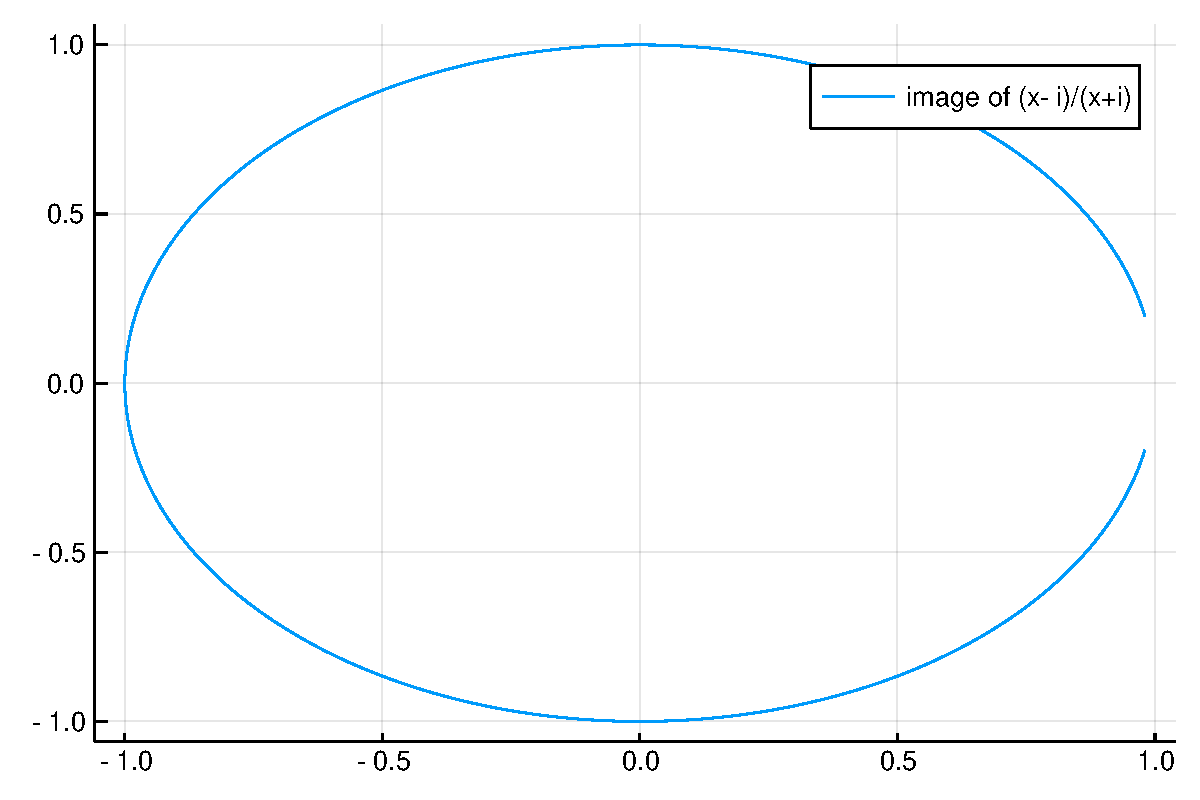
\includegraphics[width=\linewidth]{figures/Lecture25_1_1.pdf}

Therefore, $\log g(x)$ has a branch cut if we use the standard branch, which breaks the continuity requirement:


\begin{lstlisting}
(*@\HLJLnf{plot}@*)(*@\HLJLp{(}@*)(*@\HLJLn{xx}@*)(*@\HLJLp{,}@*) (*@\HLJLn{real}@*)(*@\HLJLoB{.}@*)(*@\HLJLp{(}@*)(*@\HLJLn{log}@*)(*@\HLJLoB{.}@*)(*@\HLJLp{(}@*)(*@\HLJLn{g}@*)(*@\HLJLoB{.}@*)(*@\HLJLp{(}@*)(*@\HLJLn{xx}@*)(*@\HLJLp{))))}@*)
(*@\HLJLnf{plot!}@*)(*@\HLJLp{(}@*)(*@\HLJLn{xx}@*)(*@\HLJLp{,}@*) (*@\HLJLn{imag}@*)(*@\HLJLoB{.}@*)(*@\HLJLp{(}@*)(*@\HLJLn{log}@*)(*@\HLJLoB{.}@*)(*@\HLJLp{(}@*)(*@\HLJLn{g}@*)(*@\HLJLoB{.}@*)(*@\HLJLp{(}@*)(*@\HLJLn{xx}@*)(*@\HLJLp{))))}@*)
\end{lstlisting}

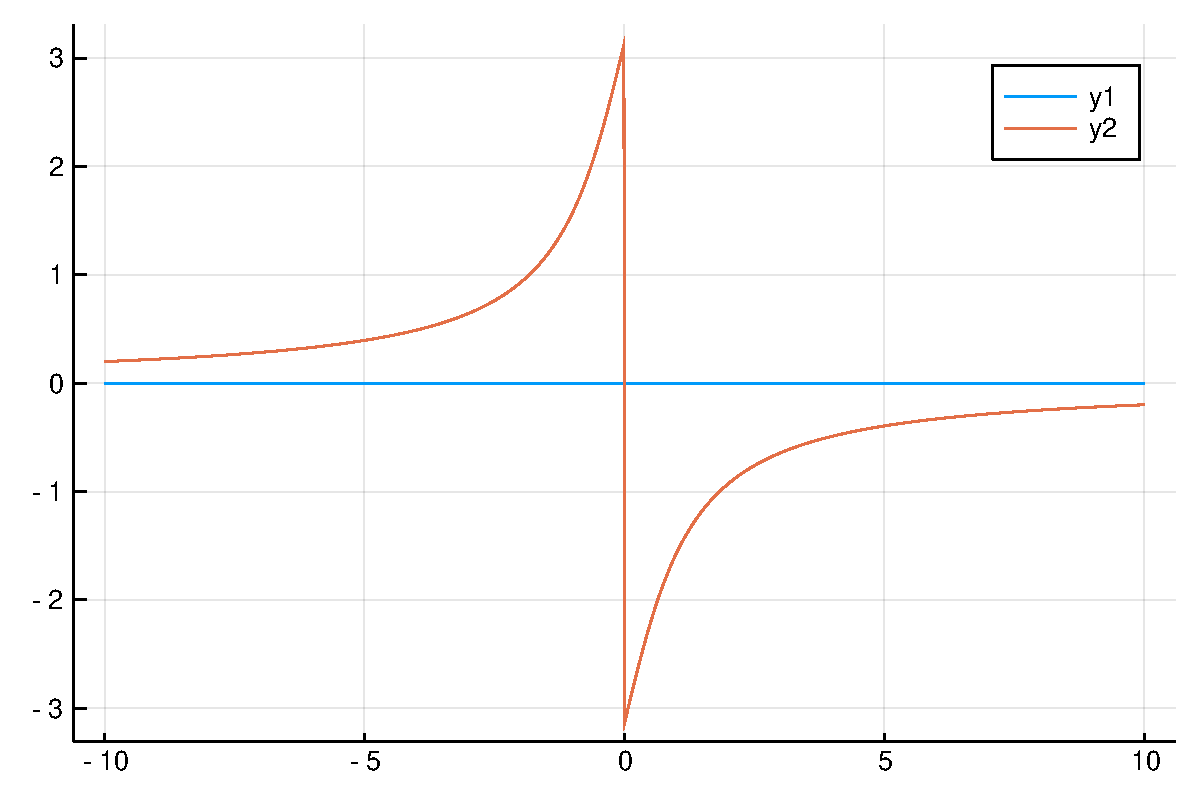
\includegraphics[width=\linewidth]{figures/Lecture25_2_1.pdf}

We could have analytically continued $\log g(z)$ using

\[
\log_1 z = \begin{cases} \log z & \Im z > 0 \\
                            \log_+ z & z < 0 \\
                            \log z + 2\pi \I & \Im z < 0 
                            \end{cases}
\]
But then $\lim_{x\rightarrow + \infty} \log_1 g(x) = 2 \pi \I$:


\begin{lstlisting}
(*@\HLJLn{log\ensuremath{\_1}}@*) (*@\HLJLoB{=}@*) (*@\HLJLn{z}@*) (*@\HLJLoB{->}@*) (*@\HLJLnf{imag}@*)(*@\HLJLp{(}@*)(*@\HLJLn{z}@*)(*@\HLJLp{)}@*) (*@\HLJLoB{>}@*) (*@\HLJLni{0}@*) (*@\HLJLoB{?}@*) (*@\HLJLnf{log}@*)(*@\HLJLp{(}@*)(*@\HLJLn{z}@*)(*@\HLJLp{)}@*) (*@\HLJLoB{:}@*) (*@\HLJLnf{log}@*)(*@\HLJLp{(}@*)(*@\HLJLn{z}@*)(*@\HLJLp{)}@*)(*@\HLJLoB{+}@*)(*@\HLJLni{2}@*)(*@\HLJLn{\ensuremath{\pi}}@*)(*@\HLJLoB{*}@*)(*@\HLJLn{im}@*)
(*@\HLJLnf{plot}@*)(*@\HLJLp{(}@*)(*@\HLJLn{xx}@*)(*@\HLJLp{,}@*) (*@\HLJLn{real}@*)(*@\HLJLoB{.}@*)(*@\HLJLp{(}@*)(*@\HLJLn{log\ensuremath{\_1}}@*)(*@\HLJLoB{.}@*)(*@\HLJLp{(}@*)(*@\HLJLn{g}@*)(*@\HLJLoB{.}@*)(*@\HLJLp{(}@*)(*@\HLJLn{xx}@*)(*@\HLJLp{))))}@*)
(*@\HLJLnf{plot!}@*)(*@\HLJLp{(}@*)(*@\HLJLn{xx}@*)(*@\HLJLp{,}@*) (*@\HLJLn{imag}@*)(*@\HLJLoB{.}@*)(*@\HLJLp{(}@*)(*@\HLJLn{log\ensuremath{\_1}}@*)(*@\HLJLoB{.}@*)(*@\HLJLp{(}@*)(*@\HLJLn{g}@*)(*@\HLJLoB{.}@*)(*@\HLJLp{(}@*)(*@\HLJLn{xx}@*)(*@\HLJLp{))))}@*)
\end{lstlisting}

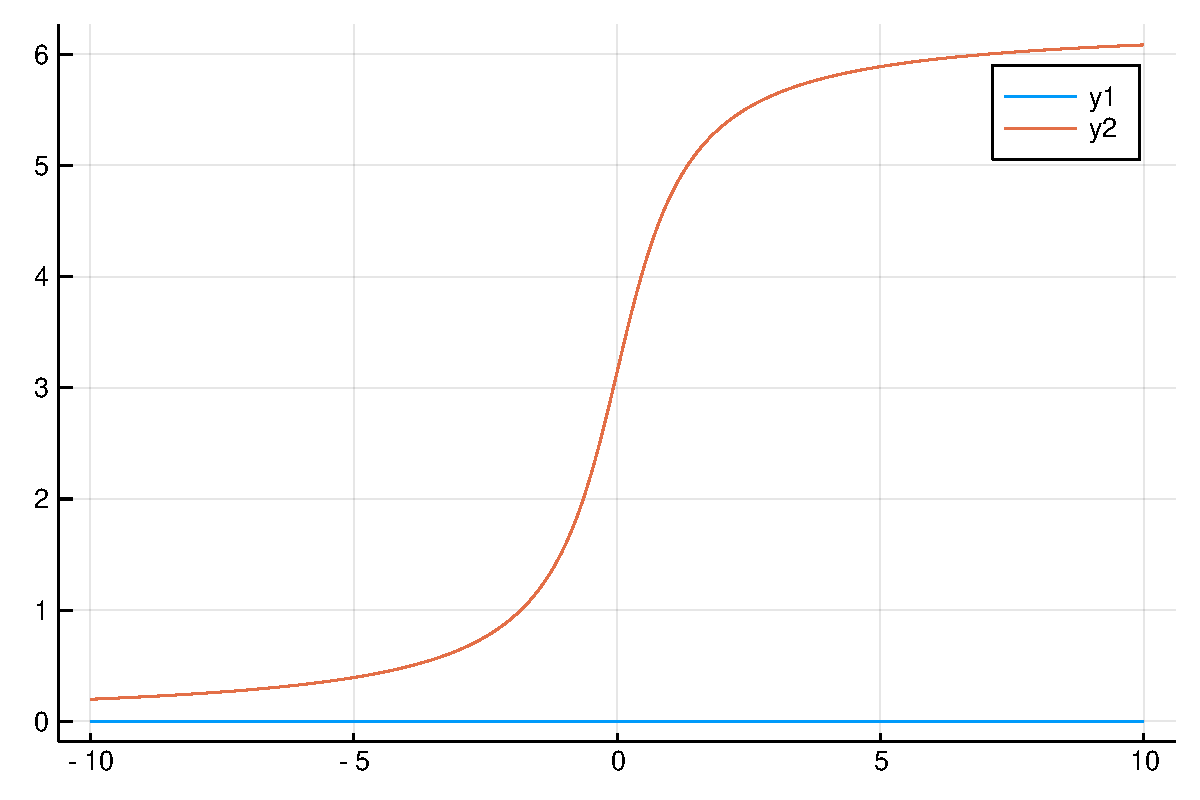
\includegraphics[width=\linewidth]{figures/Lecture25_3_1.pdf}

\textbf{Example} Consider 

\[
g(x) = {x^2+3 \over x^2+1} = 1 + O(x^{-1})
\]
Before we do anything \emph{Verify that the winding number is zero}.

We provide two methods for calculating $\Phi$: one guesses the solution, the other uses the solution formula.

\emph{Method 1 (Guess and check / kernel factorization)} If we can guess the solution, we can check it satisfies the right criteria.   Factoring $g$ we see immediately that

\[
g(x) = {x-\I \over x-\sqrt{3} \I} {x+\I \over x+\sqrt{3} \I}
\]
Note that the first term is analytic in  the upper half plane. The second term is analytic in the lower half plane \emph{and} invertible. Therefore we can guess the solution is 

\[
\Phi(z)  = \begin{cases}
        {z+\sqrt 3\I \over z+\I} & \Im z > 0 \\
            {z-\I \over z-\sqrt 3\I} & \Im z < 0
           \end{cases}
\]
This satisfies the four conditions:

\begin{itemize}
\item[1. ] Analyticity: $\Phi$ is analytic off $\R$


\item[2. ] Asymptotics: $\lim_{z\rightarrow \infty}\Phi(z) = 1$ 


\item[3. ] Weaker than pole singularities


\item[4. ] It has the right jump

\end{itemize}
\[
g(x) \Phi_-(x) =  {x^2+3 \over x^2+1} {x-\I \over x-\sqrt 3\I}  = {x+\I \over x+\sqrt 3 \I} = \Phi_+(x)
\]
This function is indeed analytic off the real line.

\emph{Method 2 (evaluate explicit form)} This is real valued and positive, hence the winding number of its image is zero.  We have 

\[
\log g(x) = \log({x+\sqrt 3\I \over x+\I}{x-\sqrt 3\I \over x-\I}) 
\]
Because they are complex conjugates, we know $\log a \bar a = \log a + \log \bar a$ as $[1, \bar a, a]$ lies in the same half plane for $a = {s+\sqrt 3 \I \over s+ \I}$, therefore we can expand:

\[
\log g(x) = \log{x+\sqrt 3\I \over x+\I} + \log {x-\sqrt 3\I \over x-\I}
\]
Now we note that $\log{x+3\I \over x+\I}$ is analytic in the upper-half plane, therefore it's Cauchy transform, by Plemelj, is

\[
\CC\br[\log{x+\sqrt 3\I \over x+\I}](z) = \begin{cases}
        \log{z+\sqrt 3\I \over z+\I} & \Im z > 0 \\
           0 & \Im z < 0
           \end{cases}
\]
Similarly,

\[
\CC\br[\log{x-\sqrt 3\I \over x-\I}](z) = \begin{cases}
        -\log{z-\sqrt 3\I \over z-\I} & \Im z > 0 \\
           0 & \Im z < 0
           \end{cases}
\]
We thus get:

\[
\Phi(z) = \E^{\CC\log g(z)} = \E^{\begin{cases}
        \log{z+\sqrt 3 \I \over z+\I} & \Im z > 0 \\
            -\log{z- \sqrt 3\I \over z-\I} & \Im z < 0
           \end{cases}} = \begin{cases}
        {z+ \sqrt 3 \I \over z+\I} & \Im z > 0 \\
            {z-\I \over z-\sqrt 3\I} & \Im z < 0
           \end{cases}
\]
\subsubsection{Inhomogenous Riemann\ensuremath{\endash}Hilbert problem}
Consider now the  Riemann\ensuremath{\endash}Hilbert problem with zero at infinity:

\[
\Psi_+(x) - g(x)\Psi_-(x) = f(x) \qqand \Psi(\infty) =0
\]
Consider writing $\Psi(z) =  \Phi(z) Y(z)$. Then we can reduce the Riemann\ensuremath{\endash}Hilbert problem to a subtractive problem: 

\[
\Psi_+(x) - g(x)\Psi_-(x) = \Phi_+(x)(Y_+(x) - Y_-(x))\qqand Y(\infty) = 0
\]
Thus once we have $\Phi$, we can determine $Y$ as a Cauchy transform, and thence construct $\Psi$.

What if we don't have decay? Just add in a constant times $\Phi$:

\textbf{Corollary} Suppose $\log g$ satisfies the conditions of Plemelj's theorem. Then

\[
\Psi(z) = \Phi(z) \CC_\R\br[{f \over \Phi_+}](z) + D \Phi(z)
\]
is the unique solution to

\[
\Psi_+(\zeta) - g(\zeta)\Psi_-(\zeta) = f(\zeta) \qqand \Psi(\infty) =D
\]
\emph{Example} Suppose $f(x) = {\I \over \I-x}$. 

To decompose this as a sum of things analytic in half planes, we just use partial fraction expansion!


\begin{align*}
{\I \over \I-x} {x + \I \over x+ \I \sqrt{3}} &= {\I \over \I-x}{2\I \over \I(1+ \sqrt{3})}  +{\I \over \I(1+\sqrt 3)} {\I(1-\sqrt 3) \over x+ \I \sqrt{3}}\\
&= \underbrace{{-2 \I \over x-\I}{1 \over 1+ \sqrt{3}}}_{-Y_-(x)}  + \underbrace{{\I \over 1+\sqrt 3} {1-\sqrt 3 \over x+ \I \sqrt{3}}}_{Y_+(x)}
\end{align*}
Thus we get

\[
Y(z) = \begin{cases} 
{\I \over 1+\sqrt 3} {1-\sqrt 3 \over z+ \I \sqrt{3}} & \Im z > 0 \\
{2 \I \over z-\I}{1 \over 1+ \sqrt{3}} & \Im z < 0
\end{cases}
\]
Let's double check: We thus have the solution:


\begin{align*}
\Psi(z)  &= \Phi(z) \CC_\R\br[{f \over \Phi_+}](z) = \begin{cases} 
{\I \over 1+\sqrt 3} {1-\sqrt 3 \over z+ \I \sqrt{3}} {z+\sqrt{3}\I \over z+\I} & \Im z > 0 \\
{2 \I \over z-\I}{1 \over 1+ \sqrt{3}} {z-\I \over z-\sqrt{3}\I} & \Im z < 0
\end{cases} \\
    &= \begin{cases} 
{\I \over 1+\sqrt 3} {1-\sqrt 3 \over z+\I} & \Im z > 0 \\
{2 \I  \over 1+ \sqrt{3}} {1 \over z-\sqrt{3}\I} & \Im z < 0
\end{cases}
\end{align*}
Let's verify it's the right thing:

\begin{itemize}
\item[1. ] It's analytic off $\R$

\end{itemize}

\begin{lstlisting}
(*@\HLJLn{\ensuremath{\Psi}}@*) (*@\HLJLoB{=}@*)  (*@\HLJLn{z}@*) (*@\HLJLoB{->}@*) (*@\HLJLnf{imag}@*)(*@\HLJLp{(}@*)(*@\HLJLn{z}@*)(*@\HLJLp{)}@*) (*@\HLJLoB{>}@*) (*@\HLJLni{0}@*) (*@\HLJLoB{?}@*) (*@\HLJLn{im}@*)(*@\HLJLoB{*}@*)(*@\HLJLp{(}@*)(*@\HLJLni{1}@*)(*@\HLJLoB{-}@*)(*@\HLJLnf{sqrt}@*)(*@\HLJLp{(}@*)(*@\HLJLni{3}@*)(*@\HLJLp{))}@*)(*@\HLJLoB{/}@*)(*@\HLJLp{(}@*)(*@\HLJLni{1}@*)(*@\HLJLoB{+}@*)(*@\HLJLnf{sqrt}@*)(*@\HLJLp{(}@*)(*@\HLJLni{3}@*)(*@\HLJLp{))}@*)(*@\HLJLoB{/}@*)(*@\HLJLp{(}@*)(*@\HLJLn{z}@*)(*@\HLJLoB{+}@*)(*@\HLJLn{im}@*)(*@\HLJLp{)}@*) (*@\HLJLoB{:}@*)
                       (*@\HLJLni{2}@*)(*@\HLJLn{im}@*)(*@\HLJLoB{/}@*)(*@\HLJLp{((}@*)(*@\HLJLn{z}@*)(*@\HLJLoB{-}@*)(*@\HLJLnf{sqrt}@*)(*@\HLJLp{(}@*)(*@\HLJLni{3}@*)(*@\HLJLp{)}@*)(*@\HLJLoB{*}@*)(*@\HLJLn{im}@*)(*@\HLJLp{)}@*)(*@\HLJLoB{*}@*)(*@\HLJLp{(}@*)(*@\HLJLni{1}@*)(*@\HLJLoB{+}@*)(*@\HLJLnf{sqrt}@*)(*@\HLJLp{(}@*)(*@\HLJLni{3}@*)(*@\HLJLp{)))}@*)

(*@\HLJLnf{phaseplot}@*)(*@\HLJLp{(}@*)(*@\HLJLoB{-}@*)(*@\HLJLnfB{3..3}@*)(*@\HLJLp{,}@*) (*@\HLJLoB{-}@*)(*@\HLJLnfB{3..3}@*)(*@\HLJLp{,}@*) (*@\HLJLn{\ensuremath{\Psi}}@*)(*@\HLJLp{)}@*)
\end{lstlisting}

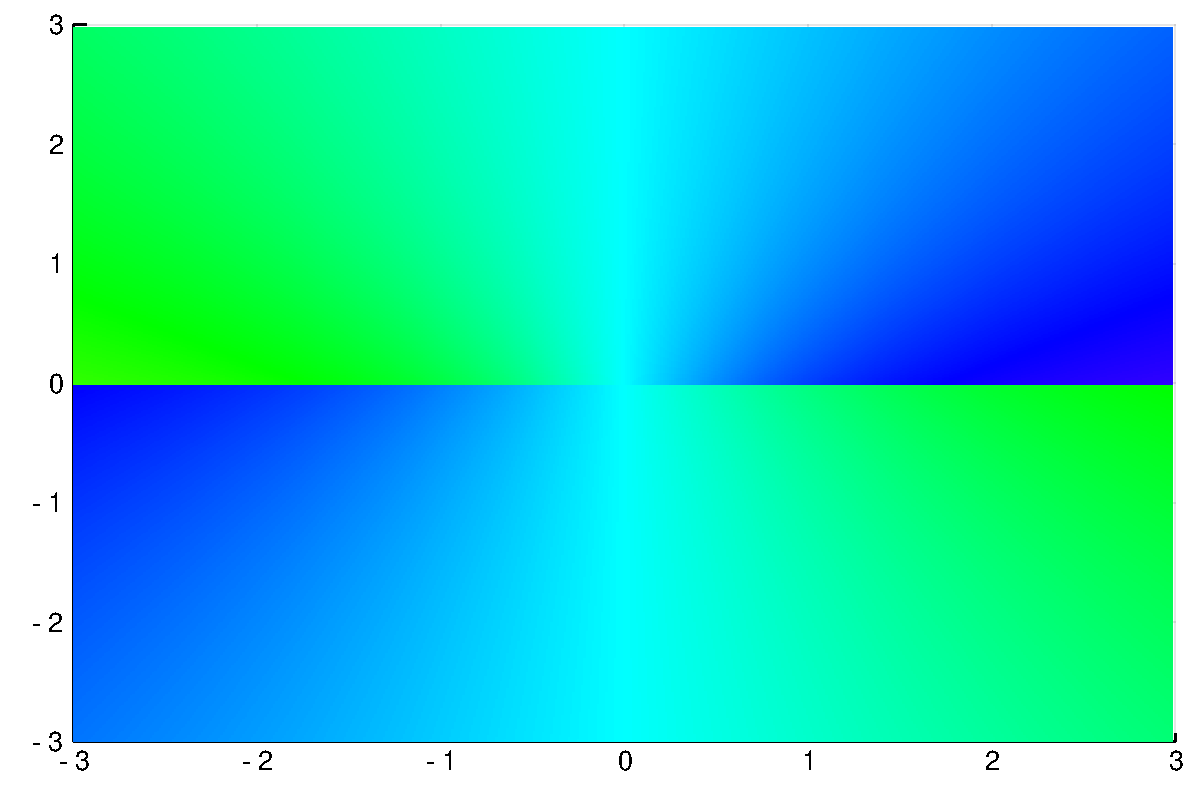
\includegraphics[width=\linewidth]{figures/Lecture25_4_1.pdf}

2. It goes to zero at infinity


\begin{lstlisting}
(*@\HLJLnf{\ensuremath{\Psi}}@*)(*@\HLJLp{(}@*)(*@\HLJLnfB{300.0}@*)(*@\HLJLoB{+}@*)(*@\HLJLnfB{300.0}@*)(*@\HLJLn{im}@*)(*@\HLJLp{)}@*)
\end{lstlisting}

\begin{lstlisting}
-0.0004465795146304169 - 0.0004450958617578906im
\end{lstlisting}


3. It satisfies the right jump:


\begin{align*}
 \Psi_+(x) - g(x) \Psi_-(x) = {\I \over 1+\sqrt 3} {1-\sqrt 3 \over x+\I}  - {x^2 + 3 \over x^2 + 1} 
{2 \I  \over 1+ \sqrt{3}} {1 \over x-\sqrt{3}\I}  \\
 = {\I (x-\I) \over 1+\sqrt 3} {1-\sqrt 3 \over x^2+1}  - {x + \sqrt{3} \I \over x^2 + 1} 
{2 \I  \over 1+ \sqrt{3}}  \\
= {1\over x^2 + 1} 
{1 \over 1+ \sqrt{3}}  \left(\I(1-\sqrt 3) x+1-\sqrt{3}  - 2\I x + 2 \sqrt{3}    \right) \\
= {1\over x^2 + 1} 
 \left(-\I x+1    \right) = {\I \over \I - x}
\end{align*}

\begin{lstlisting}
(*@\HLJLn{f}@*) (*@\HLJLoB{=}@*) (*@\HLJLn{x}@*) (*@\HLJLoB{->}@*) (*@\HLJLn{im}@*)(*@\HLJLoB{/}@*)(*@\HLJLp{(}@*)(*@\HLJLn{im}@*)(*@\HLJLoB{-}@*)(*@\HLJLn{x}@*)(*@\HLJLp{)}@*)
(*@\HLJLn{g}@*) (*@\HLJLoB{=}@*) (*@\HLJLn{x}@*) (*@\HLJLoB{->}@*) (*@\HLJLp{(}@*)(*@\HLJLn{x}@*)(*@\HLJLoB{{\textasciicircum}}@*)(*@\HLJLni{2}@*)(*@\HLJLoB{+}@*)(*@\HLJLni{3}@*)(*@\HLJLp{)}@*)(*@\HLJLoB{/}@*)(*@\HLJLp{(}@*)(*@\HLJLn{x}@*)(*@\HLJLoB{{\textasciicircum}}@*)(*@\HLJLni{2}@*)(*@\HLJLoB{+}@*)(*@\HLJLni{1}@*)(*@\HLJLp{)}@*)
(*@\HLJLnf{\ensuremath{\Psi}}@*)(*@\HLJLp{(}@*)(*@\HLJLnfB{0.1}@*)(*@\HLJLoB{+}@*)(*@\HLJLnf{eps}@*)(*@\HLJLp{()}@*)(*@\HLJLn{im}@*)(*@\HLJLp{)}@*) (*@\HLJLoB{-}@*) (*@\HLJLnf{\ensuremath{\Psi}}@*)(*@\HLJLp{(}@*)(*@\HLJLnfB{0.1}@*)(*@\HLJLoB{-}@*)(*@\HLJLnf{eps}@*)(*@\HLJLp{()}@*)(*@\HLJLn{im}@*)(*@\HLJLp{)}@*)(*@\HLJLoB{*}@*)(*@\HLJLnf{g}@*)(*@\HLJLp{(}@*)(*@\HLJLnfB{0.1}@*)(*@\HLJLp{)}@*) (*@\HLJLoB{-}@*) (*@\HLJLnf{f}@*)(*@\HLJLp{(}@*)(*@\HLJLnfB{0.1}@*)(*@\HLJLp{)}@*)
\end{lstlisting}

\begin{lstlisting}
-1.1102230246251565e-16 + 2.7755575615628914e-17im
\end{lstlisting}



\end{document}
